\subsection{Idea general}

Un primer intento para conseguir una solución a este problema es utilizando un algoritmo goloso. La idea del mismo es sencilla, numeramos los nodos de $1$ a $n$, y luego tomando de a uno los agregamos a alguno de los conjuntos de $1$ a $k$ intentando que sume a la solución el menor peso posible.

Mas formalizado el algoritmo quedará de la siguiente manera:


\begin{algorithm}
  \begin{algorithmic}[1]\parskip=1mm
 \caption{ Goloso()}
 		\STATE{Numero los vertices de $1$ a $n$} 
		\STATE{Creo una cantidad $k$ de conjuntos donde iré guardando vertices}
 		\STATE{Para cada nodo $i$ de $1$ a $n$: }
		\STATE{\quad Para cada conjunto}
			\STATE{\quad\quad Sumo todos los pesos de las aristas de ($i$,$j$) con $j$ los vertices que estan en el conjunto}
 		\STATE{\quad Agrego la el vertice $i$ para el cual la suma dio menor}
		\STATE{Imprimo por salida estandar la respuesta}
  \end{algorithmic}
  \end{algorithm}


Claramente este algoritmo no devuelve la solución exacta, y como se verá mas adelante, la solución que devuelve puede estar tan lejos como se quiera de la optima, lo que lo hace un algoritmo no muy bueno.

El analisis de complegidad es sencillo, se itera por cada vertice sobre cada conjunto. Dado que cada nodo solo estará en un conjunto, entre todos los conjuntos a lo sumo tendrán $n$ nodos, lo que hace que se deba iterar $n$ veces a lo sumo sobre $n$ nodos, luego la complegidad será $O(n^2)$, por lo que, al menos en lo que respecta a tiempos, es ampliamente superior que el algoritmo exacto.

Por lo tanto, dada la baja complegidad de este algoritmo, podría utilizarse como una cota superior, si bien algo grosera, para la solución.

\subsection{Problemas del Algoritmo Goloso}

Como ya adelantamos, la solución para este algoritmo no siempre da una solución exacta, y puede ser tan mala como se quiera. Esto surge principalmente de darle un orden a los nodos, como mostraremos en el siguiente ejemplo.

Supongamos que tenemos un grafo como el que se muestra en la figura y $K = 2$

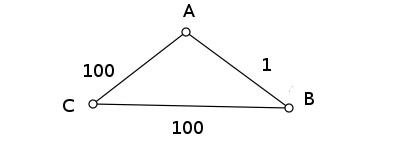
\includegraphics[scale=0.5]{Ej3/grafo.png}

Es claro que la mejor solución posible es poner en uno de los conjuntos a $A$ y $B$ y en el otro a $C$, así la suma intrapartición es $1$.

Sin embargo, supongamos que nuestro algoritmo goloso toma como primer nodo al nodo $A$, dado que no hay otros nodos, lo agrega en cualquiera de los dos conjuntos y se obtiene peso $0$. Ahora supongamos que el algoritmo toma el nodo $B$, si lo pone en el mismo conjunto que el nodo $A$ obtiene peso $1$, si lo pone en el otro conjunto obtiene peso $0$, asi que lo pone en el otro conjunto. Pero ahora falta agregar el nodo $C$, y agregandolo en cualquiera de los dos conjuntos se obtiene peso $100$. Asi que la solución para k-PMP que encontrará el algoritmo goloso será $100$.
De ahí se desprende que cambiando ambos pesos $100$ por cualquier valor puede obtenerse una solución tan mala como uno quiera.

Sin embargo, puede observarse otra cosa de este algoritmo, si se hubiese tomado el nodo $C$ como primer nodo o como segundo nodo, se hubiera llegado a la solución optima. De aquí surge la idea de que si se eligieran diferentes ordenes para los nodos y se corriera el algoritmo para cada uno de estos ordenes, podría obtenerse diferentes cotas, y con un poco de suerte en alguna de ellas no sucederá este caso que acabamos de ver.

Esta idea la utilizaremos mas adelante para el GRASP, correremos con distintos ordenes de nodos el algoritmo goloso de manera tal de obtener en cada una de estas iteraciones una respuesta diferente y posiblemente mejor que la anterior.